% !Mode:: "TeX:UTF-8:Main"
\documentclass{article}
\usepackage[utf8]{inputenc} %probably not needed ...
\usepackage[T1]{fontenc}
\usepackage{geometry}
\geometry{papersize={128mm,96mm},margin=0.5cm} %\textwidth=11.8, \textheight=8.6
\usepackage[x11names,svgnames]{xcolor}
\usepackage{tikz}
\usetikzlibrary{backgrounds}
\usepackage{tikzducks}

\tikzset{alphorn/.pic={
\begin{scope}[y=0.80pt, x=0.80pt,
yscale=-1,xshift=-91.05,yshift=-437.82]
    % path1940
    \path[draw=black,fill=brown,line join=miter,line cap=butt,miter limit=4.00,even
      odd rule,line width=2.400pt] (172.6512,452.4520) .. controls
      (193.9102,456.5182) and (215.7505,462.9100) .. (235.7835,462.0722) .. controls
      (260.8621,454.7203) and (286.4738,436.8879) .. (313.5464,390.3218) --
      (555.5536,36.1797) -- (565.9253,42.2925) -- (383.2350,357.3613) --
      (322.8158,458.1640) .. controls (311.7991,476.3000) and (296.6711,493.6138) ..
      (278.9821,510.4153) .. controls (231.2668,545.7757) and (181.1216,536.1601) ..
      (126.6548,511.5759) -- (172.6512,452.4520) -- cycle;

    % path3714
    \path[draw=black,fill=white,line join=miter,line cap=butt,miter limit=4.00,even
      odd rule,line width=2.400pt] (556.0253,29.2491) -- (558.7568,30.8313) --
      (569.6826,37.1600) -- (572.4141,38.7422) .. controls (573.9410,39.6267) and
      (570.7767,45.0896) .. (569.2497,44.2052) -- (566.5183,42.6230) --
      (555.5924,36.2942) -- (552.8610,34.7120) .. controls (551.3340,33.8276) and
      (554.4984,28.3646) .. (556.0253,29.2491) -- cycle;

    % path6371
    \path[draw=black,fill=white,line join=miter,line cap=butt,miter limit=4.00,even
      odd rule,line width=2.400pt] (188.4619,454.7661) -- (181.1482,463.1063) --
      (143.2906,506.1125) -- (133.8263,516.8640) .. controls (128.5354,522.8744) and
      (115.3166,511.8355) .. (120.6073,505.8252) -- (130.0716,495.0738) --
      (167.9293,452.0676) -- (175.2428,443.7273) .. controls (180.5217,437.7074) and
      (193.7408,448.7462) .. (188.4619,454.7661) -- cycle;

    % path8143
    \path[draw=black,fill=white,line join=miter,line cap=butt,miter limit=4.00,even
      odd rule,line width=2.400pt] (208.1255,467.1077) -- (203.9668,484.7697);

    % path8145
    \path[draw=black,fill=white,line join=miter,line cap=butt,miter limit=4.00,even
      odd rule,line width=2.400pt] (219.4993,471.0159) -- (218.6225,489.4545);

    % path8147
    \path[draw=black,fill=white,line join=miter,line cap=butt,miter limit=4.00,even
      odd rule,line width=2.400pt] (233.0026,468.6109) -- (241.0946,480.9868);

    % path8149
    \path[draw=black,fill=white,line join=miter,line cap=butt,miter limit=4.00,even
      odd rule,line width=2.400pt] (249.3118,480.6110) -- (271.0073,510.0477);

    % path8151
    \path[draw=black,fill=white,line join=miter,line cap=butt,miter limit=4.00,even
      odd rule,line width=2.400pt] (236.7856,487.1748) -- (252.3182,518.3651);

    % path8153
    \path[draw=black,fill=white,line join=miter,line cap=butt,miter limit=4.00,even
      odd rule,line width=2.400pt] (225.4368,491.3335) -- (230.8732,525.6804);

    % path8155
    \path[draw=black,fill=white,line join=miter,line cap=butt,miter limit=4.00,even
      odd rule,line width=2.400pt] (210.0295,493.7385) -- (206.3718,528.3360);

    % path8157
    \path[draw=black,fill=white,line join=miter,line cap=butt,miter limit=4.00,even
      odd rule,line width=2.400pt] (195.4991,486.7990) -- (184.6513,525.0541);
 \end{scope}
}}

\definecolor{swissred}{RGB}{216,30,5}
\tikzset{swisscross/.pic={
\begin{scope}[y=0.80pt, x=0.80pt,
yscale=-1,yshift=-240]
%\path[fill=swissred,rounded corners=0.0000cm] (0.0000,0.0000) rectangle
%  (300.0000,300.0000);
\path[fill=white,rounded corners=0.0000cm] (50.0000,120.0000) rectangle
  (250.0000,180.0000);
\path[fill=white,rounded corners=0.0000cm] (120.0000,50.0000) rectangle
  (180.0000,250.0000);
\end{scope}
}}

\usepackage{eso-pic}
\begin{document}
\AddToShipoutPictureBG{%
 \begin{tikzpicture}[overlay,remember picture]

 \fill[DeepSkyBlue](current page.north west) rectangle (current page.south east);
 \fill[white] (current page.west)--([yshift=-1cm]current page.north)--(current page.east)-- (current page.south east)-- (current page.south west)--cycle;

 \fill[white] (current page.west)--([yshift=-1cm]current page.north)--(current page.east)-- (current page.south east)-- (current page.south west)--cycle;

 \begin{scope}
 \path[clip] (current page.south west) --++(0,7)--++(\paperwidth,0)--++(0,-7) --cycle;
 \fill[ForestGreen] (current page.west)--([yshift=-1cm]current page.north)--(current page.east)-- (current page.south east)-- (current page.south west)--cycle;

 \end{scope}
 \end{tikzpicture}}


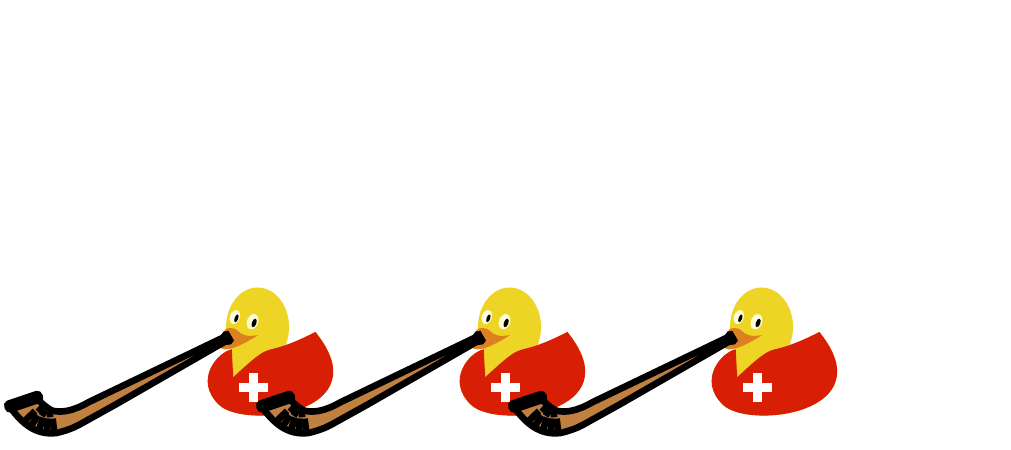
\begin{tikzpicture}
\path[use as bounding box](-2.2,0)--++(0,5cm)--++(\textwidth,0);
\begin{scope}[scale=0.8,transform shape]
\duck[jacket=swissred]
\draw([xshift=-3.7cm,yshift=-1.2cm]bill) pic[scale=0.2,transform shape,rotate=-30] {alphorn};
\draw([yshift=-0.5cm, xshift=-0.3cm]wing) pic[scale=0.08]{swisscross};
\end{scope}

\begin{scope}[scale=0.8,transform shape,xshift=4cm]
\duck[jacket=swissred]
\draw([xshift=-3.7cm,yshift=-1.2cm]bill) pic[scale=0.2,transform shape,rotate=-30] {alphorn};
\draw([yshift=-0.5cm, xshift=-0.3cm]wing) pic[scale=0.08]{swisscross};
\end{scope}

\begin{scope}[scale=0.8,transform shape,xshift=8cm]
\duck[jacket=swissred]
\draw([xshift=-3.7cm,yshift=-1.2cm]bill) pic[scale=0.2,transform shape,rotate=-30] {alphorn};
\draw([yshift=-0.5cm, xshift=-0.3cm]wing) pic[scale=0.08]{swisscross};
\end{scope}

\begin{scope}[transform shape,xshift=1.5cm, yshift=-3cm]
\duck[jacket=swissred]
\draw([xshift=-3.7cm,yshift=-1.2cm]bill) pic[scale=0.2,transform shape,rotate=-30] {alphorn};
\draw([yshift=-0.5cm, xshift=-0.3cm]wing) pic[scale=0.08]{swisscross};
\end{scope}

\begin{scope}[transform shape,xshift=5cm,yshift=-3cm]
\duck[jacket=swissred]
\draw([xshift=-3.7cm,yshift=-1.2cm]bill) pic[scale=0.2,transform shape,rotate=-30] {alphorn};
\draw([yshift=-0.5cm, xshift=-0.3cm]wing) pic[scale=0.08]{swisscross};
\end{scope}


\end{tikzpicture}

\begin{tikzpicture}

\end{tikzpicture}



\end{document}


\path(current bounding box.north east);
\pgfgetlastxy{\XCoord}{\YCoord};
\fill[red,overlay] (current bounding box.north east)circle(2pt)node[above] {\XCoord,\YCoord};
\path(current bounding box.south west);
\pgfgetlastxy{\XCoord}{\YCoord};
\fill[red,overlay] (current bounding box.south west) circle(2pt)node[above] {\XCoord,\YCoord};
